\chapter{My Appendix}

In \cref{sec:generalbound}, we provide a detailed proof of the general Lieb-Robinson-type bound for long-range interactions with $\al\le D$ mentioned in Eq.~(15) of the main text. The bound has a closed-form expression that can be used to lower bound the signaling time [see Eq.~(16)] for $\al \le D$.

In \cref{sec:exactsumbound}, we derive a second general Lieb-Robinson-type bound that is the tightest one can get from the Lieb-Robinson series mentioned in Eq.~(13), although it lacks a closed-form analytic expression.
We show numerically that the signaling time obtained from this bound has the same scaling as a function of system size $N$ as the bound in Eq.~(15) of the main text when $N$ is sufficiently large.
Therefore, the bound presented in the main text is\dash in a broad sense\dash the best one can obtain without developing new techniques beyond those used in deriving the traditional Lieb-Robinson series.

\section{Proving the general Lieb-Robinson-type bound for $\al \le D$}
\label{sec:generalbound}
Before we present the proof of the general Lieb-Robinson-type bound given in Eq.~(15) of the main text, let us summarize in \cref{sec:math} some mathematical preliminaries useful for the proof.

\subsection{Mathematical preliminaries}
\label{sec:math}
In this section, we elaborate on the scaling of the on-site hop parameter $J_{ii}$ defined after Eq.~(14).
We define the quantity $\lambda = \max_{i\in\Lambda} J_{ii}$, which for power-law interactions has strength
\begin{equation}
	\label{eq:self-hop}
	\lam = \max_{i\in\Lam} \sum_{j\in\Lam\backslash i} J_{ij} = \max_{i\in\Lam}\sum_{j\in\Lam\backslash i} \frac{1}{r_{ij}^{\al}}.
\end{equation}
If the lattice $\Lam$ is a square lattice with unit spacings, then $\lambda$ scales as
\begin{equation}
        \label{eq:lamdef2}
	\lam = \begin{cases}
        \Th{N^{1-\al/D}} & \text{for }0\le\al<D,\\
        \Th{\log N} & \text{for }\al=D,\\
        \Th 1 & \text{for }\al>D.
\end{cases}
\end{equation}
In general, the scaling of $\lam$ as a function of $N$ in \cref{eq:lamdef2} holds asymptotically for large regular lattices \cite{Storch15}.

For $\al \le D$, we note that $\lam$ diverges in the thermodynamic limit.
For some applications, it is preferred to apply a normalizing factor of $1/\lam$ (due to Kac \cite{Kac63}) to the Hamiltonian to ensure the system energy is extensive. Since experimental systems (such as those with dipolar interactions in 3D) do not necessarily have extensive energy, we would prefer not to apply the Kac normalization. The light cone contours for Kac-normalized Hamiltonians follow straightforwardly from our results upon rescaling the time by a factor of $\lambda$.

In the rest of this subsection, we justify the dependence of $\lambda$ on $N$ and $\al$ as shown in \cref{eq:lamdef2}.
We assume that the lattice $\Lam$ is $D$-dimensional with $N = L^D$ sites.
Without loss of generality, let $i$ be the site located at the origin and define $r_j \equiv r_{ij} \ge 1$.
For $0\le \al < D$, we bound \cref{eq:self-hop} above by an integral:
\begin{align}
	\sum_{j\in\Lam} \frac{1}{r_{j}^{\al}} &\le \int_{\vec{r}\in \mathbb{R}^D} \frac{d^D\vec{r}}{\|\vec{r}\|^\al}
	= \frac{2\pi^{\frac D 2}}{\Gamma(\frac D2)} \int_0^L \frac{dr}{r^{\al-D+1}}  = \frac{\omega_D}{D-\al}L^{D-\al},
\end{align}
where $\omega_D\equiv 2\pi^{\frac D 2}\big/\Gamma(\frac{D}{2})$ is the hyper-surface area of a unit $D$-sphere and $\Gamma(\cdot)$ is the Gamma function.  It follows that $\lam = \O{ N^{1-\al/D}}$  for $\al<D$.
The asymptotic lower bound $\lam = \W{N^{1-\al/D}}$ follows from setting $\|\vec r\| \rightarrow \|\vec r\| +\sqrt D$ and integrating from $r=1$ to $r=\infty$.

For $\al = D$, we perform the same calculation, taking care to avoid integrating over the origin:
\begin{align}
	\sum_{j\in\Lam} \frac{1}{r_{j}^{\al}} &\le  \int_{\|\vec{r}\| \ge 1} \frac{d^D\vec{r}}{\|\vec{r}\|^D} + \sum_{j \in \Lam} \theta \left( 1+\sqrt{D} - r_j\right)
    \\ & \le  \omega_D \int_1^L \frac{dr}{r} + \frac{\omega_D\left(1+\sqrt D+\frac12\right)^D}{\omega_D\left(\frac12\right)^D}
    \\ &= \frac {\omega_D}D \log(N) + \left(2\sqrt D+3\right)^D,
\end{align}
where $\theta(\cdot)$ denotes the Heaviside step function. So, at the critical point $\al=D$, we have $\lam = \O{ \log(N)}$.
The lower bound $\lam = \W{\log(N)}$ holds in a similar fashion.

For $\al > D$, the sum in \cref{eq:self-hop} converges, so $\lam$ can be bounded by a constant independent of $N$.
Thus, we have verified the asymptotic scaling of the on-site parameter $\lam$ for the three cases listed in  \cref{eq:lamdef2}.

\subsection{Proof of the bound in Eq.~(15)}
\label{sec:newbound}

In this section, we provide a simple proof of Eq.~(15) for long-range interactions.
First, let us recall the Lieb-Robinson series from Eq.~(13) of the main text.
\begin{align}
	\label{eq:HKseries2}
		\|[A(t),B]\| &\le 2\|A\|\|B\||X||Y|\sum_{k=1}^{\infty}\frac{(2t)^{k}}{k!} \J^k(X,Y), \\
	\label{eq:hopping2}
	\J^k(X,Y) &\equiv \sum_{i_{1},\dots,i_{k-1}}J_{Xi_{1}}J_{i_{1}i_{2}}\dots J_{i_{k-1}Y}.
\end{align}
We use the so-called \emph{reproducibility condition} for finite systems with power-law decaying interactions \cite{HK, Gong14}. Specifically, for $\al > 0$ and distinct $i,j\in \Lam$, the second-order hopping term $k=2$ in \cref{eq:hopping2} can be bounded by
\begin{equation}
	\label{eq:repcon}
	\J^2(i,j) = \sum_k J_{ik}J_{kj} \le p\lam J_{ij},
\end{equation}
where $p=2^{\al+1}$ and $\lam$ is the on-site hop parameter defined in \cref{eq:self-hop}.
This inequality allows the power-law decay of $J_{ij}$ to be reproduced across multiple hopping terms.

We reorder the summations on the right-hand side of \cref{eq:hopping2} by introducing a new index $n$ to count the number of self-hops in a particular sequence of hopping sites $\{i_1,\dots,i_{k-1}\}$.
Specifically, $n$ represents the number of indices $j\in\{0,\dots,k-1\}$ such that $i_{j}=i_{j+1}$ (with $i_{0}=X$ and $i_{k}=Y$).
Now let us first assume that the $n$ self-hops occur in the first $n$ terms ($J_{Xi_1}$ to $J_{i_{n-1}i_{n}}$). Then we may rewrite the right-hand side of \cref{eq:hopping2} as
%
\begin{equation}
\label{eq:selfhopresum}
\sum_{i_{1},\dots,i_{k-1}}J_{Xi_{1}}\dots J_{i_{k-1}Y}
= \lambda^n \sum_{i_{n+1},\dots,i_{k-1}}J_{i_{n}i_{n+1}}\dots J_{i_{k-1}Y},
\end{equation}
%
using the fact that each self-hop term $J_{ii}$ is equal to $\lam$.
If, on the other hand, the $n$ self-hops appear in arbitrary positions in the sequence of hops, then accounting for these cases multiplies \cref{eq:selfhopresum} by the combinatorial factor of $\binom k n$.
Inserting into \cref{eq:hopping2} gives
%
\begin{align}
	\label{eq:choose}
	\J^k(X,Y) = \sum_{n=0}^{k}{\binom k n}\lambda^{n} \left[\sum_{i_{n+1},\dots,i_{k-1}}J_{i_Xi_{n+1}}\dots J_{i_{k-1}Y} \right],
\end{align}
where we relabeled $i_n$ as $X$.
Now, using the fact that $i_{j}\neq i_{j+1}$ for $j=n,\dots,k-1$ (where $i_k=Y$), we can apply the reproducibility condition in \cref{eq:repcon} a total of $k-n$ times along with the normalization condition $J_{ij} = 1/r_{ij}^{\al}$ for $i\neq j$ to get
%
\begin{align}
	\sum_{i_{n+1},\dots,i_{k-1}}J_{Xi_{n+1}}\dots J_{i_{k-1}Y} \le (\lam p)^{k-n-1} J_{XY} = \frac{(\lam p)^{k-n-1}}{r_{XY}^{\al}}.
\end{align}
%
Finally, inserting this inequality into \cref{eq:choose} and applying the binomial theorem gives
\begin{equation}
\mathcal{J}^{k}(r_{XY}) \le \sum_{n=0}^{k}{\binom k n}\lambda^{n}\left[\frac{(\lambda p)^{k-n-1}}{r_{XY}^{\al}}\right]\ = \frac{(\lambda+\lambda p)^{k}}{\lambda pr_{XY}^{\al}}.
\end{equation}
Inserting this bound for $\mathcal{J}^{k}(r_{XY})$ into \cref{eq:HKseries2} gives an exponential series bound for the commutator
\begin{align}
	\|[A(t),B]\| &\le 2\|A\|\|B\||X||Y|\sum_{k=1}^{\infty}\frac{(2t)^{k}}{k!} \J^k(X,Y) \\
    &\le 2\|A\|\|B\||X||Y|\sum_{k=1}^{\infty}\frac{(2t)^{k}}{k!} \frac{(\lambda(1+p))^{k}}{\lambda pr_{XY}^{\al}}\\
    &= 2\|A\|\|B\||X||Y| \left(\frac{e^{2\lam t(1+p)}-1}{\lambda pr_{XY}^{\al}}\right) \\
    &= 2\|A\|\|B\||X||Y|\left(\frac{e^{\Theta(N^{1-\al/D})t}-1}{\Theta(N^{1-\al/D})r_{XY}^\al}\right), \label{eq:newbound2}
\end{align}
which reproduces Eq.~(15) in the main text.


% \section{Second general Lieb-Robinson-type bound for $\al \le D$}
\label{sec:exactsumbound}
The above derivation of the bound in \cref{eq:newbound2} requires the use of the reproducibility condition~[\cref{eq:repcon}], which can make the bound loose compared to the Lieb-Robinson series in \cref{eq:HKseries2}. In this section, we will exactly sum the series in \cref{eq:HKseries2} and compare the resulting bound to that of \cref{eq:newbound2}. We will show by numerical analysis that\dash although the bound obtained directly from the Lieb-Robinson series is tighter than the one \cref{eq:newbound2}\dash it largely shares the same scaling behavior when the number of sites $N$ is large.

\subsection{Summing the Lieb-Robinson series exactly}
\label{sec:exactsumboundproof}
We now exactly calculate the sum in \cref{eq:HKseries2} without using the reproducibility condition. Since \cref{eq:HKseries2} is an infinite series, one cannot perform the sum directly. But using a discrete Fourier transform, the series can be summed numerically in a highly efficient manner.

To use the discrete Fourier transform, we assume that $J_{ij}=1/r_{ij}^\al$ is translationally invariant. Note that the physical interaction strength between lattice sites does not need to be translationally invariant, as it just needs to be bounded by $J_{ij}$. his additional assumption does not greatly affect the generality of the following results.

For simplicity, we consider a 1D lattice $\Lam$ that consists of $N$ spins on a ring; the following results generalize straightforwardly to lattices in arbitrary dimensions. Let $r_{ij} = \min\{|i-j|,|N-i+j|\}$ be the (periodic) distance metric, which coincides with the graph distance $d(i,j)$ on $\Lam$. Due to translational invariance, we denote $J_{ij}$ by $J(r_{ij})$ which satisfies $J(r+N) = J(r)$.

We now perform a discrete Fourier transform from the position space parameterized by $r=0,1,2,\cdots,N-1$ to a momentum space parameterized by $p=0,1,2,\cdots,N-1$, denoted by $\mathcal{F}_p[f(r)]=\sum_{r=0}^{N-1}e^{-2\pi ipr/N}f(r)$.
We observe that the sum in the definition of $\J^k(X,Y)$ in \cref{eq:hopping2} can be rewritten as the $k$-fold convolution of $J(r)$ with itself.
Thus, letting $r\equiv r_{XY}$ and $\J^k(r) \equiv J^k(X,Y)$, the discrete Fourier transform of \cref{eq:hopping2} is given by
\begin{align}
	\mathcal{F}_p[\J^{k}(r)]  = \omega(p)^k,
\end{align}
where $\omega(p)=\mathcal{F}_p[J(r)]$.
We now take the discrete Fourier transform of the entire series in \cref{eq:HKseries2}:
\begin{align}
\mathcal{F}_p\left[	\|[A(t),B]\|\right] & \le\sum_{k=1}^{\infty}\frac{(2t)^{k}}{k!}\omega(p)^k = e^{2\omega(p)t}-1. \label{eq:fcomm}
\end{align}
The series in \cref{eq:HKseries2} can thus be evaluated exactly by taking the inverse Fourier transform of \cref{eq:fcomm}:
%
\begin{equation}
	\label{eq:exactbound}
		\|[A(t),B]\| \le \mathcal{F}_r^{-1}\left[e^{2\omega(p) t}-1\right].
\end{equation}
where $\mathcal{F}_r^{-1}[g(p)]\equiv\frac{1}{N}\sum_{p=0}^{N-1}e^{2\pi ipr/N}g(p)$ defines the inverse discrete Fourier transform.
For $\al = 0$, the inverse Fourier transform can be evaluated to yield the analytical expression \begin{equation}
    \|[A(t),B]\| \leq 2\|A\|\|B\||X||Y|\left(\frac{e^{4Nt}-1}{N}\right),
\end{equation}
which matches the bound in \cref{eq:newbound2} up to constant factors.
For $\al > 0$, it is difficult to obtain a simple analytical expression for the bound in \cref{eq:exactbound}. We will thus evaluate this bound numerically, as detailed in the next section.

\subsection{Numerical comparison of the two bounds}
\label{exactboundnumerics}

In this section, we study the asymptotic scaling of the exact summation bound in \cref{eq:exactbound}.
Because the discrete Fourier transform can be performed rather efficiently using the Fast Fourier Transform algorithm \cite{FFT65} numerically, we can evaluate the right-hand side of \cref{eq:exactbound} for system sizes up to the order of $10^6$.
This allows us to compare the bound in \cref{eq:exactbound} (referred to below as the ``exact summation bound") with the bound in \cref{eq:newbound2} (referred to below as the ``analytical bound") for large $N$.

Let us first focus on the large-$r$ asymptotic behavior of the two bounds.
As a typical example, we set $N = 10^6$ and $t = 1/\lam$ and plot the right-hand side of the two bounds (with $\|A\|=\|B\|=|X|=|Y|=1$) as a function of $r$ for $\al = 0.5$ in \cref{Fig_Rdep}.
Unsurprisingly, the right-hand side of the analytic bound in \cref{eq:newbound2} decays as $1/r^{\al}$ for the entire range of $r$.
The exact summation bound leads to the same scaling for small $r$, but not for large $r$.
While this comparison leaves room for potential tightening of the bound in \cref{eq:newbound2} for large $r$, generic improvement of the bound for all $r$ seems unlikely.

\begin{figure}[h]
	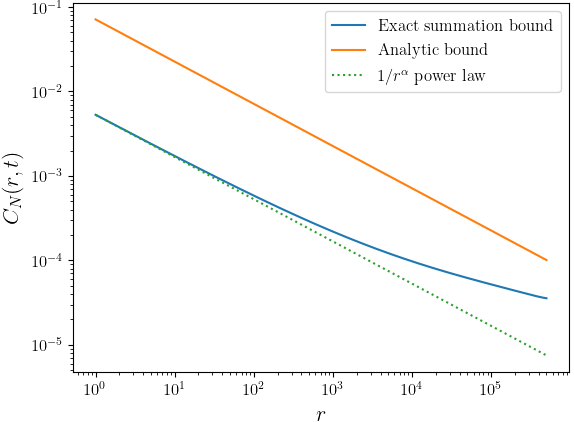
\includegraphics[width=.5\linewidth]{figures/Rdep.png}
    \caption{A comparison between the exact summation bound [\cref{eq:exactbound}] and the analytical bound [\cref{eq:newbound2}] sites as a function of the distance $r$ between operators $A$ and $B$. The specific plot assumes a 1D periodic lattice with $N = 10^6$, $\al = 0.5$, $t = 1/\lam$, and $r=1,2,\cdots,N/2$.}
    \label{Fig_Rdep}
\end{figure}

Next, we compare the $N$-dependence of the two bounds. To get rid of the $r$-dependence, we will compare the signaling times between two sites with either $r=1$ (the smallest possible separation on a 1D ring) or $r=N/2$ (the largest possible separation).
If the two bounds agree with each other at both $r=1$ and $r=N/2$ in the large $N$ limit, it is reasonable to believe that they will agree with each other at all values of $r$.

For $\al < 1$, the analytical bound gives the following signaling time (upon setting $\|[A(t),B]\|= 1$) as function of $r$ and $N$:
\begin{equation}
	\label{eq:contour_al<D}
	t_\text{si}(r,N) =\W{\frac{\log(N^{1-\al}r^{\al})}{N^{1-\al}}}.
\end{equation}
Choosing either $r=1$ or $r=N$ leads to $t_\text{si}=\Omega(N^{\al-1}\log(N))$, consistent with Eq.~(16) of the main text. For the exact summation bound, we numerically compute $t_\text{si}$ by finding the value of $t$ that makes $\|[A(t),B]\| = 1$ over a range of $N$ from $10^4$ to $10^6$ for both $r = 1$ and $r = N/2$. We then fit $t$ as a function of $N$ to the function $a N^\gamma \log(N)$.
\begin{figure*}[h]
	\subfigure[~$r = 1$]{
	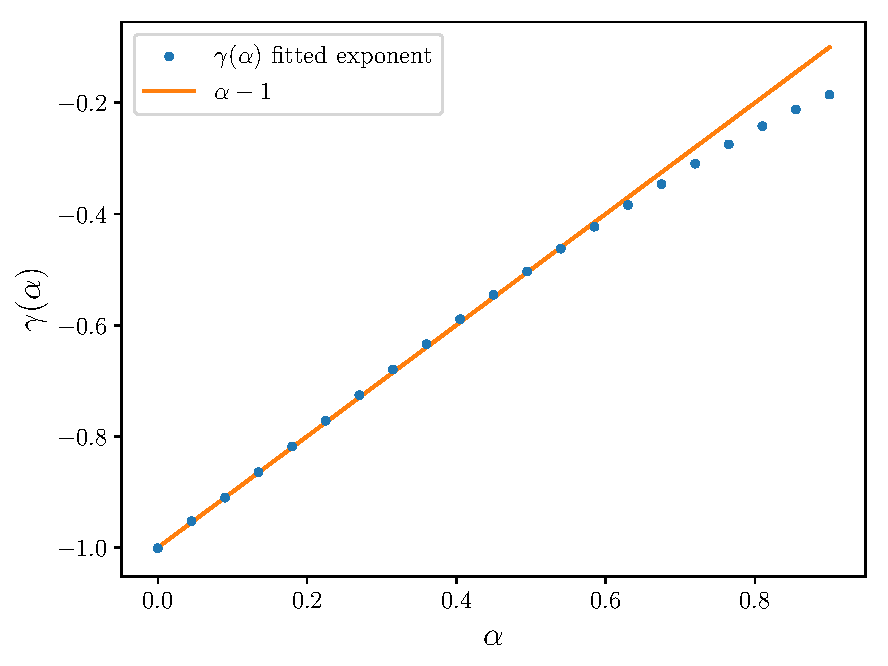
\includegraphics[width=.45\textwidth]{figures/beta_0.pdf}
    } \qquad
    \subfigure[~$r = N/2$]{
    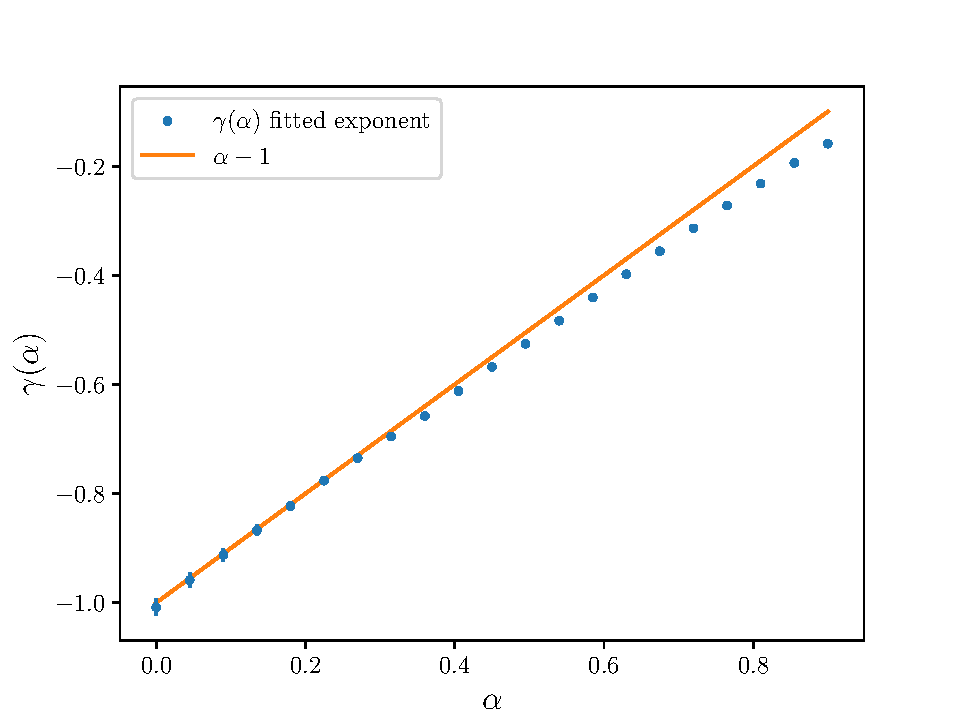
\includegraphics[width=.455\textwidth]{figures/beta_1.pdf}}
	\caption{The fitted exponent $\gamma$ in the signaling time scaling obtained from the exact summation bound in \cref{eq:exactbound} at $r=1$ (a) and $r=N/2$ (b) for $a\in [0,1]$. The error bars reflect the 95\% confidence intervals for the fit.}
        \label{Fig_al<D}
\end{figure*}
In \cref{Fig_al<D}, we plot the fitted exponent $\gamma(\al)$ as a function of $\al$. We observe that $\gamma(\al)$ scales approximately as $\al-1$ as long as $\al$ is not close to 1 for both $r=1$ and $r=N$, showing that both bounds lead to approximately the same scaling of signaling time in $N$.

When $\al\rightarrow 1$, $\gamma(\al)$ deviates from $\al-1$ noticeably. We attribute such deviation to finite-$N$ effects in our numerical evaluation of the exact summation bound. In particular, we notice that as $\al\rightarrow 1$, $\lambda$ (which plays an important role in both bounds) is not well-approximated by $N^{\al-1}$ for insufficiently large enough $N$. For such values of $N$, $\lambda$ is better approximated by $\log(N)$.

To give further clarification, we perform a comparison of the two bounds exactly at $\al=1$, where we can exactly use $\log(N)$ in place of $N^{\al-1}$. The signaling time given by the analytical bound now scales as
\begin{equation}
	t_\text{si}(r,N) = \W{\frac{\log(r\log N)}{\log N}}.\label{eq:scalinga1}
\end{equation}
We then fit the signaling time obtained from the exact summation bound at $\al=1$ using the above scaling function and find very good agreement between the two bounds. For example, at $r=1$ the signaling time from the exact summation bound can be fitted by the function $ a\:\log(N)^b\:\log\log(N)^c$ with $b=-1.0$ and $c=0.95$, which agrees with the scaling of $\log\log(N)/\log(N)$ provided by \cref{eq:scalinga1}. As a result, we expect the signaling time bounds given by both bounds to have the same scaling in $N$ when the system size is large enough for all $\al\le D$.
